Given the transfer function, \begin{align}
    H(s) = \frac{1}{s+2}\\
    \implies \frac{Y(s)}{X(s)} = \frac{1}{s+2}
\end{align}
and input signal,
\begin{align}
    x(t) = 10u(t)
\end{align}
By applying Laplace transform
\begin{align}
    \mathcal{L}\{x\}(s)=10\mathcal{L}\{u\}(s)
\end{align}
We know that Laplace transform of unit step function ($u(t)$) is $\frac{1}{s}$ (discussed in class) 
\begin{align}
    X(s) &= \frac{10}{s}\\
    \implies Y(s) &= \frac{10}{s(s+2)}\\
    \implies Y(s) &= 5\brak{\frac{1}{s}-\frac{1}{s+2}}
\end{align}
Applying inverse Laplace transform on $Y(s)$ for output signal $y(t)$
\begin{align}
    y(t) &= \mathcal{L}^{-1}\{Y(s)\}(t)\\
    \implies y(t) &= 5(1-e^{-2t})
\end{align}
So the steady state value of output signal is 5. Time taken to reach 99\% of its steady state value will be
\begin{align}
    5(1-e^{-2t}) &= (0.99)5\\
    \implies e^{-2t} &= 0.01\\
    \implies t &= 2.3sec
\end{align}
\begin{figure}[!ht]
    \centering
    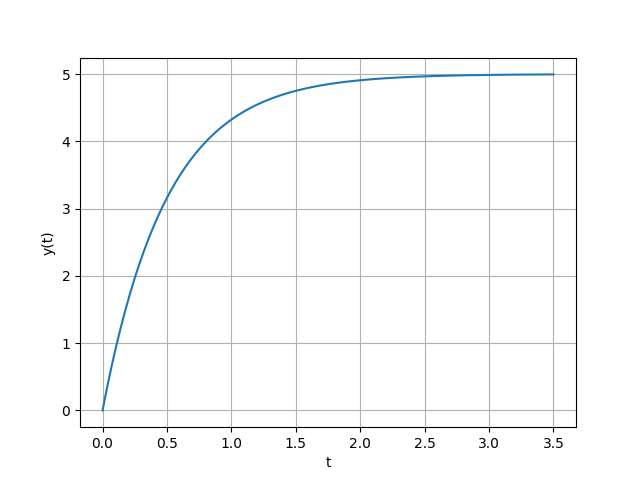
\includegraphics[width=\columnwidth]{solutions/ec/2004/64/figures/simulated_plot.png}
    \caption{Simulated plot of output signal y(t)}
    \label{ec/2004/64/plot}
\end{figure}
